\chapter{The Simplex Method}
\section{Linear Programs and Polyhedra}
A linear program in general has the form:
\begin{eqnarray*}
\text{minimize:}& \vec c \cdot \vec x \\
\text{subject to:} & A \cdot \vec x \geq \vec b
\end{eqnarray*}
where $x=\trans{(\nthings{x})}$ is an vector of variables in $\R$. $x$ together with the vector $c \in \R^n$ define the objective function. Note that in this script the cost vector is always a row vector. Should you find formulas with $\trans c$ in them think hard if that's actually right and mail the authors if not.

$A \in \R^{m \times n}$ together with $x\in \R^m$ and $b \in \R^m$ form the system of inequalities which describe the constraints.

\subsection*{Standard Form}\label{Sec:standardForm}
A LP in standard form\footnote{Cormen et al. call this slack-form (Schlupfform)} is of the form:
\begin{eqnarray*}
\text{minimize:}& \vec c \cdot \vec x \\
\text{subject to:} & A \cdot \vec x = \vec b \\
& x\geq0
\end{eqnarray*}

Any LP can be transformed into an equivalent LP in standard form. Two steps are needed for this, one to add non negativity constraints for all variables and a second to transform any inequalities into a equalities.

\begin{enumerate}
\item {\bfseries Add non negativity constraints:} Suppose a variable $x$ has no non-negativity constraint. $x$ can be replaced with two variables $x'$ and $x''$ such that $x=x'-x''$ and $x',x''\geq 0$, as any negative number can be written as a combination of two non negative numbers. Figure \ref{Fig:1dTo2d} shows the transformation of the one dimensional LP:
\begin{eqnarray*}
\text{minimize:}& x \\
\text{subject to:} & x \geq -2\\
& x \leq 4
\end{eqnarray*}

\begin{figure}[hbt]
\begin{minipage}[hbt]{0.4\linewidth}
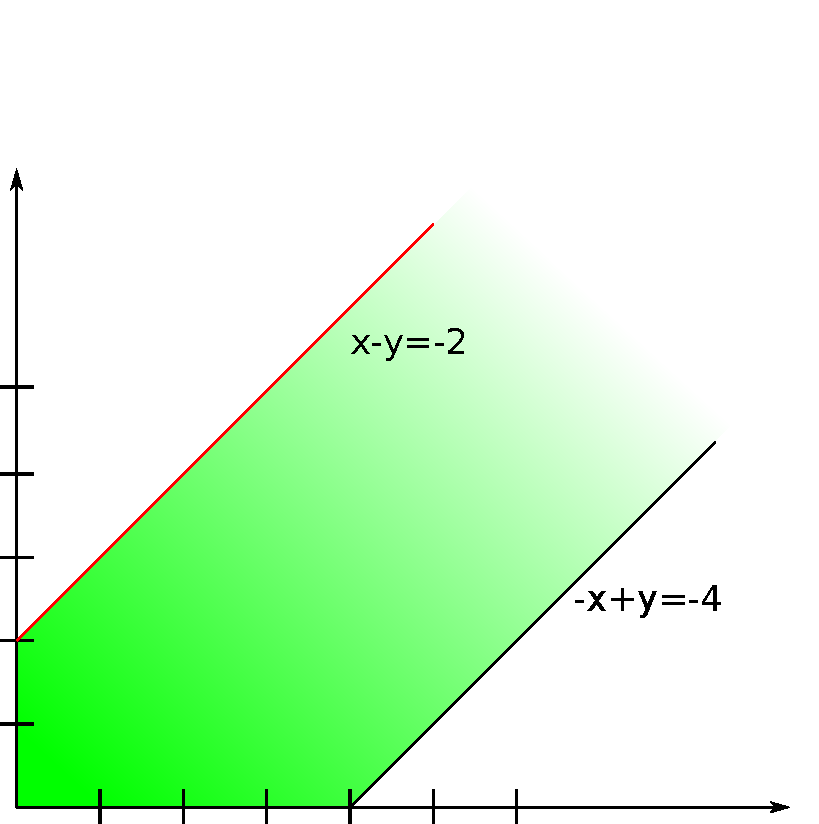
\includegraphics[width=1\textwidth]{./images/1dTo2d.pdf}
\end{minipage}
\hfill
\begin{minipage}[hbt]{0.4\linewidth}
\begin{align*}
\text{min: } x-y\\
x-y \geq -2\\
-x+y \geq -4\\
x,y \geq 0
\end{align*}

\end{minipage}
\caption{Adding non negativity constraints. The red line shows the optimal solutions.}
\label{Fig:1dTo2d}
\end{figure}

\item {\bfseries Remove inequalities:} Suppose a constraint $a$ to be $x_1+2x_2 \geq 15$. By adding a new variable $s\in \R$ and the constraint $a-s=15$ we can remove the inequality. So by adding a new vector $s\in \R^n$ with $A \cdot \vec x - s = \vec b$ the inequalities can be removed.
\end{enumerate}

Of course the solution we get for the LP in standard form can't be immediately used as a solution for the original LP. However the values of the original variables are easily reconstructed.

Solving LPs with just two variables is rather easy. We can use a graphical approach in two dimensions. The constraints define halfplanes in the 2D space. The feasible region of the problem, i.e. all the points that satisfy all constraints, is then the intersection of all the halfplanes. The cost vector now defines a halfspace of its own (i.e. lines with equivalent costs) that can be shifted around by choosing different $x$. If $x$ lies within the feasible region we get a feasible solution. The goal is to shift the lines as far in negative $c$ direction as possible without leaving the feasible region. See figure \ref{Fig:graphSolutionEx}.

\begin{figure}[hbt]
\begin{minipage}[hbt]{0.4\linewidth}
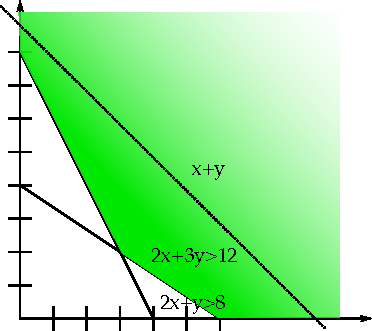
\includegraphics{./images/graphSolutionEx.pdf}
\end{minipage}
\hfill
\begin{minipage}[hbt]{0.4\linewidth}
\begin{align*}
\min & x+y\\
s.t.\quad&2x+y\geq 8\\
&2x+3y\geq 12
\end{align*}
\end{minipage}
\caption{An example for a graphical solution of an LP. The optimal solution is (3,2)}
\label{Fig:graphSolutionEx}
\end{figure}

How can we derive an algorithm from this method? We use the idea of sliding down, but just look at the corners of the feasible region, to get discrete steps (continuous sliding can't be implemented well). We start with any corner of the feasible region (a basic feasible solution) and look at its neighbors. Should they have a better objective value we move, else we're finished. 

We'll show that this method is correct, i.e. that it is enough to look at the corners of the feasible region and stop at a local minimum.

To formalize the intuition from the 2D-space we need a notion of a corner in a (usually high dimensional) feasible region. To use it in an algorithm it should be a non-graphical definition. First we give some general definitions and then three different alternative definitions of a corner. We finish by proving that they are all equivalent.

\begin{Def}[Polyhedron]\label{Def:polyhedron} A polyhedron is a set in $\R^n$ whose members obey a set of linear inequalities
\[\{x\in \R^n | Ax \geq b\} \qquad A\in \R^{m\times n},\ b\in \R^m\]
If the region is bounded (i.e. it has a finite volume) it can also be called polytope.
\end{Def}

\begin{Def}[Hyperplane, Hyperspace] \label{Def:hyperPlaneSpace} Let $a,x\in \R^n$, $a\neq 0$. 
\begin{enumerate}
\item $\{x|ax=b\}$ is a \emph{hyperplane} (a line in 2D)
\item $\{x|ax\geq b\}$ is a \emph{halfspace} (halfplane in 2D)
\end{enumerate}
\end{Def}

With definition \ref{Def:hyperPlaneSpace} we can say that a polyhedron is an intersection of a bunch of halfspaces.

\begin{Def}[Convex Sets] A subset $S \subseteq \R^n$ is called \emph{convex} if any convex combination between two points (graphically: points on a line between those points) is contained in the set. See figure \ref{Fig:convexNotConvex}
\[\forall \lambda \in [0,1], \forall x,y\in S: \lambda x + (1-\lambda) y \in S\]
\end{Def}

\begin{figure}[hbt]
\begin{center}
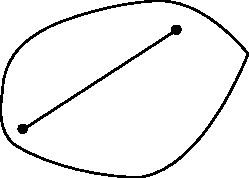
\includegraphics{./images/convex.pdf}\hspace{2cm}
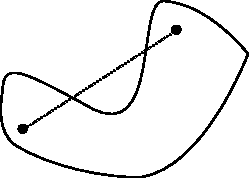
\includegraphics{./images/notConvex.pdf}
\end{center}
\caption{Graphical example for a convex and a non convex set (with non linear borders)}
\label{Fig:convexNotConvex}
\end{figure}

Convex sets have a lot of nice properties. Luckily feasible regions are always convex. This is the main reason why we can efficiently solve LPs. 

\subsection{Corners of Polyhedra}
The following definitions formalize the notion of a corner.

\begin{Def}[Vertex]\label{Def:Vertex} Let P be a polyhedron. A vector $x\in P$ is a \emph{vertex} of P if $\exists \vec c\in \R^n$
 s.t. $cx < cy$ for all $y\in P, y \neq x $; that is $x$ is the minimal point for some cost vector (the unique optimal solution for some LP with the feasible set P). See figure \ref{Fig:vertex}
\end{Def}

\begin{figure}[hbt]
\begin{center}
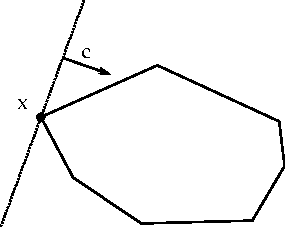
\includegraphics{./images/vertex.pdf}
\end{center}
\caption{A vertex $x$ is the optimal solution for a cost vector $c$}
\label{Fig:vertex}
\end{figure}

\begin{Def}[Extreme Point]\label{Def:ExtremePoint} An \emph{extreme point} of a polyhedron P is a vector $x\in P$ s.t. $x$ is not a convex combination of any two vectors $y,z\in P$ different from $x$. 
\end{Def}
Example: In 2D we can always select the two adjacent corners of a point $x$ on the edge of $P$ iff $x$ is not a corner. Then $x$ will be on the line between the two corners. 

\begin{Def}[Active Constraint]\label{Def:ActiveConstraint} Let $P$ be a polyhedron that is defined by some linear inequalities $a_i$: $P=\{x|a_ix\geq b_i\}$. We'll say that the $i$-th constraint is \emph{active} at a point $x$ if we have equality there $a_ix = b_i$
\end{Def}

In the constraints define the edges of polyhedron. If a point is on an edge that constraint is active. Intuitively it must be a corner if it lies on the intersection of $n$ edges.

%TODO we don't have a definition of standard form yet but the following definition is only valid for polyhedra in standard form
\begin{Def}[Basic Solution]\label{Def:BasicSolution}Let $P\in \R^n$ be a polyhedron in standard form and let $x^{*}\in \R^n$. The vector $x^{*}$ is a basic solution if all \emph{equality} constraints are active and out of the active constraints, there are $n$ of them that are linearly independent. See solution $A$ in figure \ref{Fig:bsfVSbs} for an example of a basic solution.
\end{Def}
Notice that in this definition some of the constraints of the form $x_i \geq b_i$ may be violated, as long as $n$ of them are active. In a standard form polyhedron this means that some of the $x_i \geq 0$ constraints may be violated. 

\begin{figure}[hbt]
\begin{center}
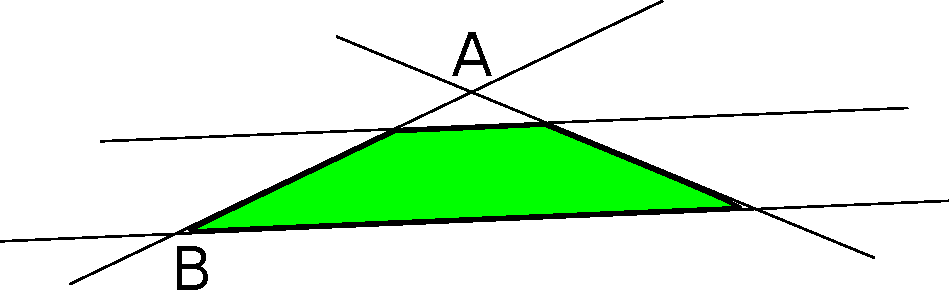
\includegraphics[width=0.5\textwidth]{./images/basicVsBasicFeasible.pdf}
\end{center}
\caption{Some LP. Solution $A$ is a basic solution. Solution $B$ is a basic feasible solution.}
\label{Fig:bsfVSbs}
\end{figure}

\begin{Def}[Basic Feasible Solution]\label{Def:BFS} Let $P$ be a polyhedron in $n$ dimensions. Then $x\in P$ is a \emph{basic feasible solution} if the set of active constraints has full rank, that is there are $n$ linearly independent active constraint vectors at the point $x$. See figure \ref{Fig:bfsActiveConstraints}. In difference to the basic solution no constraint may be violated.
\[\mbox{rank}(\{a_i\in \R^n|a_ix=b_i\}) = n\]

In particular there never is a b.f.s. if we have less than $n$ constraints. See the point $B$ in figure \ref{Fig:bsfVSbs} for an example of a basic feasible solution.
\end{Def}

\begin{figure}[hbt]
\begin{center}
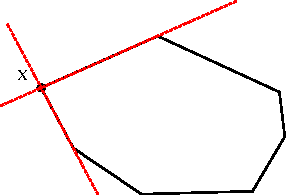
\includegraphics{./images/bfs.pdf}
\end{center}
\caption{Two constraints (red lines) are active at $x$ and it's in the feasible region. It's a basic feasible solution}
\label{Fig:bfsActiveConstraints}
\end{figure}

Now we want to prove that the three definitions \ref{Def:Vertex}, \ref{Def:ExtremePoint} and \ref{Def:BFS} are all equivalent to each other.

\begin{thm} \label{Thm:cornerEquiv} Let $P$ be a polyhedron and $x\in P$. The following statements are equivalent
\begin{enumerate}
\item $x$ is a vertex\label{enu:corner1}
\item $x$ is an extreme point\label{enu:corner2}
\item $x$ is a basic feasible solution\label{enu:corner3}
\end{enumerate}
\end{thm}

\begin{pr}[Theorem \ref{Thm:cornerEquiv}] The proof takes three steps. We show \ref{enu:corner1} $\Rightarrow$ \ref{enu:corner2} $\Rightarrow$ \ref{enu:corner3} $\Rightarrow$ \ref{enu:corner1}.
\begin{itemize}
\item vertex $\Rightarrow$ extreme point: Proof by contraposition. Assume the existence of $y,z \in P$ s.t. $y,z\neq x$ with $x= \lambda y + (1-\lambda )z$. That is, $x$ is not an extreme point because it can be expressed as a convex combination of $y$ and $z$ (definition \ref{Def:ExtremePoint}). We want to show that it's not a vertex either.

From definition of a vertex (def. \ref{Def:Vertex}) we know that some cost vector $c$ should exist such that $c x < c \lambda y  + c (1-\lambda) z$, that is $x$ is optimal w.r.t. $c$. That however is a contradiction to the assumption $x= \lambda y + (1-\lambda )z$.

\begin{align*}
cx &= \lambda cy +(1-\lambda)cz\\
   &> \lambda cx + (1-\lambda)cx = cx && \text{since }cx\leq cy, cx\leq cz\\
\end{align*}

\item extreme point $\Rightarrow$ bsf (proof by contraposition; we show $\neg \text{bsf} \Rightarrow \neg \text{extreme point}$): Suppose $x\in P$ is not a basic feasible solution. Let $B$ be a matrix of active constraints at $x$ and $C$ the matrix of the inactive constraints such that $Bx=d$, $Cx\gneq f$ and $A = \left[B\atop C\right]$, $b=\left[d\atop f\right]$. Since $x$ is not a bfs the matrix $B$ hasn't full rank\footnote{Note the slightly different full rank definition. In this case full rank is defined by the number of dimensions of the polyhedron, not in terms of the rows and columns of $B$.} and hence its kernel is nonempty. So we can find some vector in the kernel:

\[\exists \delta \in \R^n, \delta \neq 0:\ B\delta =0\]

See figure \ref{Fig:extremeBfs}. With $\delta$ we define two vectors:

\[y=x-\epsilon \delta \quad z = x+\epsilon \delta\]

Note that $x=(z+y)/2$. That means that $x$ is not an extreme point if $z,y \in P$, because $x$ is a convex combination of the two. Consider 

\[Bz = B(x+\epsilon \delta) = Bx + \epsilon B\delta = Bx\]

Since $B\delta = 0$ the active constraints are still active. For the inactive constraints we have some slack before we leave the polyhedron (We can move around on the red line in figure \ref{Fig:extremeBfs}). If we choose $\epsilon$ small enough we're still within. It suffices to choose $\epsilon$ such that 

\[\forall i: \epsilon |c_i z| < c_i x - f_i\qquad \vec c_i\in C,\ f_i \in \vec f\]

Hence $z$ (and analogous $y$) are still in the polyhedron and $x$ is not an extreme point.

\begin{figure}
\begin{center}
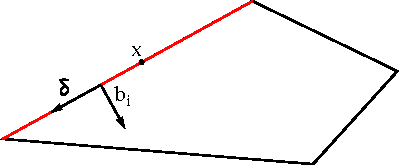
\includegraphics{./images/extreme_bfs.pdf}
\end{center}
\caption{$x$, active constraint $b_i$ and orthogonal vector $\delta$}
\label{Fig:extremeBfs}
\end{figure}

\item bfs $\Rightarrow$ vertex: Suppose $x$ is a bfs. We construct a cost vector for which $b$ is the unique optimal solution.

Let $I$ be the indices of all active constraints.Then let $c$ be the sum of the rows of $A$ that form active constrainst: and $c=\sum_{i \in I} a_i$. We know the objective value for $x$ w.r.t. $c$. It's $c x = \sum_{i \in I} b_i$, since for each $a_i x \geq b_i $, the inequality is tight (see def. \ref{Def:ActiveConstraint}). 

Also $\forall y\in P, i\in I$ we have $a_i y \geq b_i$. Therefore $c y \geq c x$. The greater then is sharp as $x$ is the unique solution to the active constraints because it's a bfs and the system of active constraints has full rank, i.e. if $n$-lines cross in $n$-dimensional space they do so at \emph{one} point. (Theorem 2.2 in the Linear Optimization book). So $x$ is the optimal solution for some LP and hence a vertex.
\end{itemize}

\end{pr}